\documentclass[uplatex,dvipdfmx]{jlreq}

\usepackage{jlreq-deluxe}
\usepackage[uplatex,deluxe]{otf} % UTF
\usepackage[noalphabet]{pxchfon} % otfの後に1回だけ読み込む
\usepackage{stix2} % 欧文＆数式フォント
\usepackage[fleqn,tbtags]{mathtools} % 数式関連
\usepackage{hira-stix} % ヒラギノフォント＆STIX2 フォント代替定義
\usepackage{float}
\usepackage[hyphens]{url} % urlパッケージ
\usepackage[
  colorlinks=false,            
  pdfborder={0 0 0}
]{hyperref}
\Urlmuskip=0mu plus 1mu  

\usepackage{tabularx}
\usepackage{array}
 \usepackage{multirow}
\usepackage{ltablex}
\keepXColumns
\renewcommand{\tabularxcolumn}[1]{m{#1}} 
\newcolumntype{C}{>{\centering\arraybackslash}X} 
\usepackage{wrapfig}
\usepackage{amsmath} 
\usepackage{mathtools} 

\usepackage{listings}
\usepackage{xcolor} % 色をつける場合

% ソースコードの見た目の設定
\lstset{
  language={C++},
  basicstyle={\ttfamily\small},
  keywordstyle={\color{blue}},
  commentstyle={\color{green!60!black}},
  stringstyle={\color{orange}},
  frame=single,          % 枠線
  breaklines=true,       % 行が長い場合に折り返す
  numbers=left,          % 行番号を左に表示
  numberstyle={\tiny},
  stepnumber=1,
  showstringspaces=false
}

\usepackage{ascmac}

\begin{document}


\title{担当箇所の基本設計・詳細設計書\_ver光同期廃止後}
\author{25G1113　廣岡花　グループ7}
\date{2026年6月22日}
\maketitle

\section{担当箇所の基本設計}
\subsection{機能一覧}
%ここにFBSを分割したもの，表を入れて詳細に説明
図\ref{fig:1-4}に担当箇所であるUIによる同期制御機能および追加の担当となったクマアニメーションを中心に詳細化したFBS図を示す．また表\ref{tab:1-3}に，各機能の概要と実装上の要点をまとめる．本システムは，1台のPC（Processing）を指揮者UI，1台のMaster Arduinoを制御ハブ，4台のSlave Arduinoを各楽器ノードとして構成し，，それぞれのSlaveに接続したPC（Processing）によって発音する．Processingから受け取った演奏設定をMasterが集約して各Slaveへ配信することで，複数ノードの演奏を協調制御する．
指揮者UI（UI.pde）は，ユーザーからの入力として，BPMの増減（[$\uparrow$]／[$\downarrow$]キー），演奏順の登録（[1]〜[3]キー），演奏順のリセット（ボタン操作），共通オクターブの増減（ボタン操作），および設定確定・送信（ボタン操作）の5種類を受け付ける．これらの入力内容は画面上の各エリアにリアルタイムに反映され，設定確定・送信ボタンが押されると，その時点のオクターブ・演奏順・BPMをまとめた1回限りの初期設定情報がMasterへ送信される．送信後は演奏中とみなし，以後はBPMの変更のみを受け付けて他の設定変更を受け付けない状態（UIロック）に切り替わる．これは，演奏中に演奏順やオクターブが変更されてしまうことを防ぐためである．
演奏制御のロックおよび解除は，Masterからの通知に基づいて行う．具体的には，Masterから演奏開始の通知（START）が送信されると，指揮者UIはBPM以外の操作を即座にロックし，演奏が終了した通知（FINISH）を受信すると，ロックを解除して通常の編集可能な状態に戻す．なお，現段階ではMaster実機との接続が無い環境での動作確認用に，キーボードの[s]キーを押すことでも同様にロックを解除できる簡易的な仕組みを設けている．
さらに，本バージョンでは指揮者UIと同一プロセス上に，BPMと演奏状態を可視化するための別ウィンドウ（BearWindow）を追加した．BearWindowは指揮者UI側から毎フレームBPMと演奏中かどうかの状態を受け取り，ドット絵画像によるクマの横スクロールアニメーションとしてこれを表示する．BPMが速いほど画面のスクロール速度が増すため，演奏のテンポを視覚的に把握できる．操作はキーボードの[Space]キーのみであり，演奏中に[Space]キーを押すとクマがジャンプし，飛んでいるコインに触れると得点（獲得コイン数）が加算される．逆に地面の障害物に接触すると，クマがダメージを受けた見た目に変化し，獲得コイン数が一定数減少する．演奏が開始されると同時に今回分の得点集計が始まり，Masterから演奏終了の通知（FINISH）を受信するとゲームを終了し，その回の獲得コイン数とこれまでの上位記録をランキングとして指揮者UI側に表示する．ただし，このランキングはProcessingの実行中のみ保持される一時的な記録であり，Processingを停止すると消去される．

\begin{figure}[H]
    \centering
    \makebox[0pt][c]{
    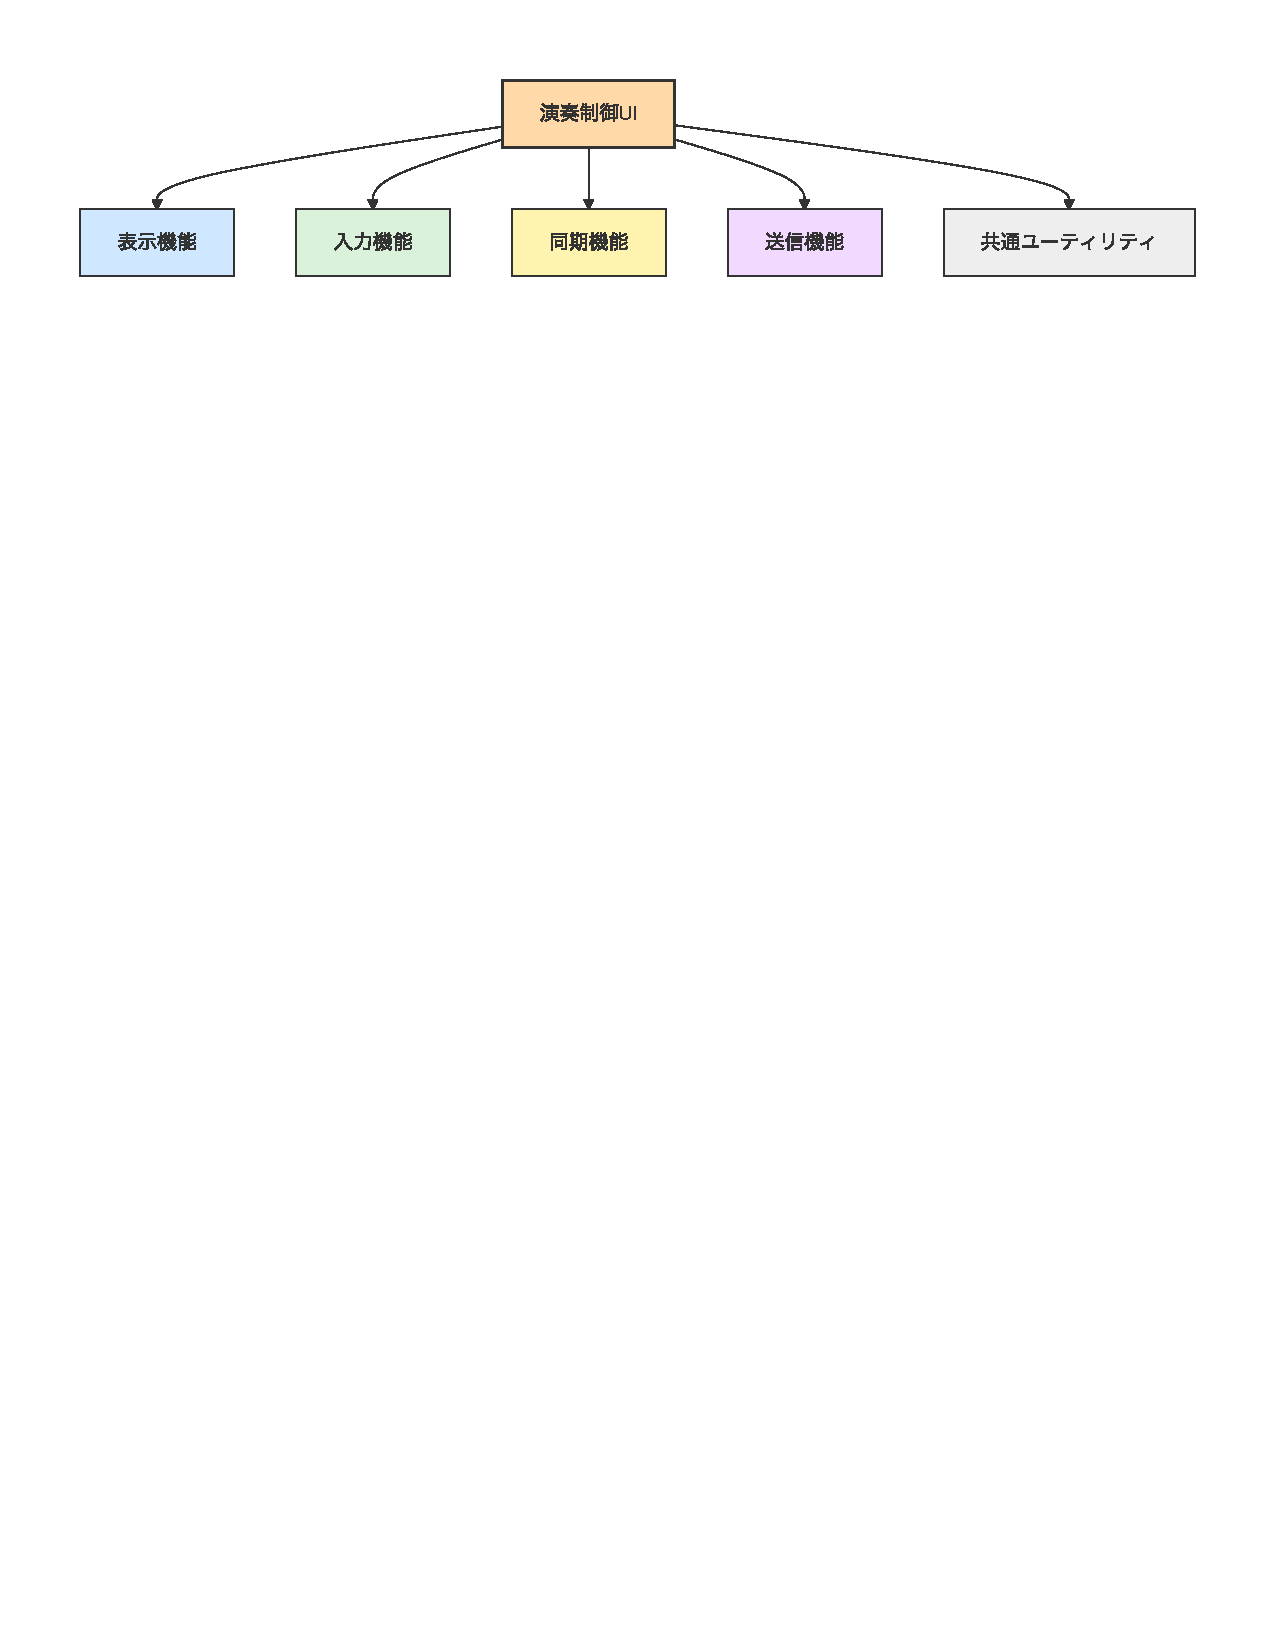
\includegraphics[width=150mm]{fig/FBS.pdf}
    }
    \caption{UI面の同期・表示に着目したFBS}
    \label{fig:1-4}
\end{figure}

\begin{table}[H]
  \centering
  \caption{演奏制御UIの機能一覧}
  \label{tab:1-3}
  \renewcommand{\arraystretch}{1.2}

  \begin{tabularx}{\linewidth}
    {|>{\centering\arraybackslash}p{3.4cm}
     |>{\raggedright\arraybackslash}X|}
    \hline
    \textbf{区分} & \textbf{内容} \\ \hline

    \multirow{6}{*}{表示機能}
      & タイトルおよび送信ボタンの描画 \\ \cline{2-2}
      & BPM設定エリアの描画 \\ \cline{2-2}
      & 演奏順番設定エリアの描画 \\ \cline{2-2}
      & 共通オクターブ設定エリアの描画 \\ \cline{2-2}
      & Slave状態ボックスの描画 \\ \cline{2-2}
      & 送信内容および現在の状態表示 \\ \hline

    \multirow{2}{*}{入力機能}
      & ↑／↓キーによるBPM変更，1\UTF{FF5E}3キーによる演奏順登録 \\ \cline{2-2}
      & 設定送信，順番リセット，オクターブ変更ボタンの操作 \\ \hline

    \multirow{3}{*}{\shortstack{演奏制御\\ロック機能}}
      & Masterから演奏開始通知（START）を受信した時点でBPM以外の操作を即座にロック \\ \cline{2-2}
      & Masterから演奏終了通知（FINISH）を受信した時点でロックを解除し，編集可能状態へ復帰 \\ \cline{2-2}
      & 実機未接続時の動作確認用として，[s]キー押下によるロック解除を仮実装 \\ \hline

    \multirow{2}{*}{送信機能}
      & オクターブ・演奏順・BPMを含む初期設定情報の生成 \\ \cline{2-2}
      & 初回の設定送信および演奏中のBPM変更送信 \\ \hline

    \multirow{2}{*}{\shortstack{共通\\ユーティリティ}}
      & ボタン領域のホバー判定 \\ \cline{2-2}
      & 演奏順および選択状態の初期化 \\ \hline

    \multirow{6}{*}{\shortstack{クマアニメー\\ション機能}}
      & ドット絵画像（歩行2種・ジャンプ・ダメージ）によるクマの表示と状態切替 \\ \cline{2-2}
      & BPMに連動したスクロール速度の制御（空・地面・雲・木・コイン・障害物） \\ \cline{2-2}
      & [Space]キーによるジャンプ操作とコイン収集 \\ \cline{2-2}
      & 障害物接触時のダメージ表示と獲得コイン数の減少 \\ \cline{2-2}
      & Masterから演奏終了通知（FINISH）受信時のゲーム終了とランキング表示（Processing停止で記録は消去） \\ \cline{2-2}
      & ランキングおよびベストスコアの保持・更新 \\ \hline

  \end{tabularx}
\end{table}

\newpage

\subsection{具体的な実装内容}
%各分割したシステムごとの具体的な実装内容

\subsubsection{UI設定入力}

\begin{figure}[H]
    \centering
    \makebox[0pt][c]{
    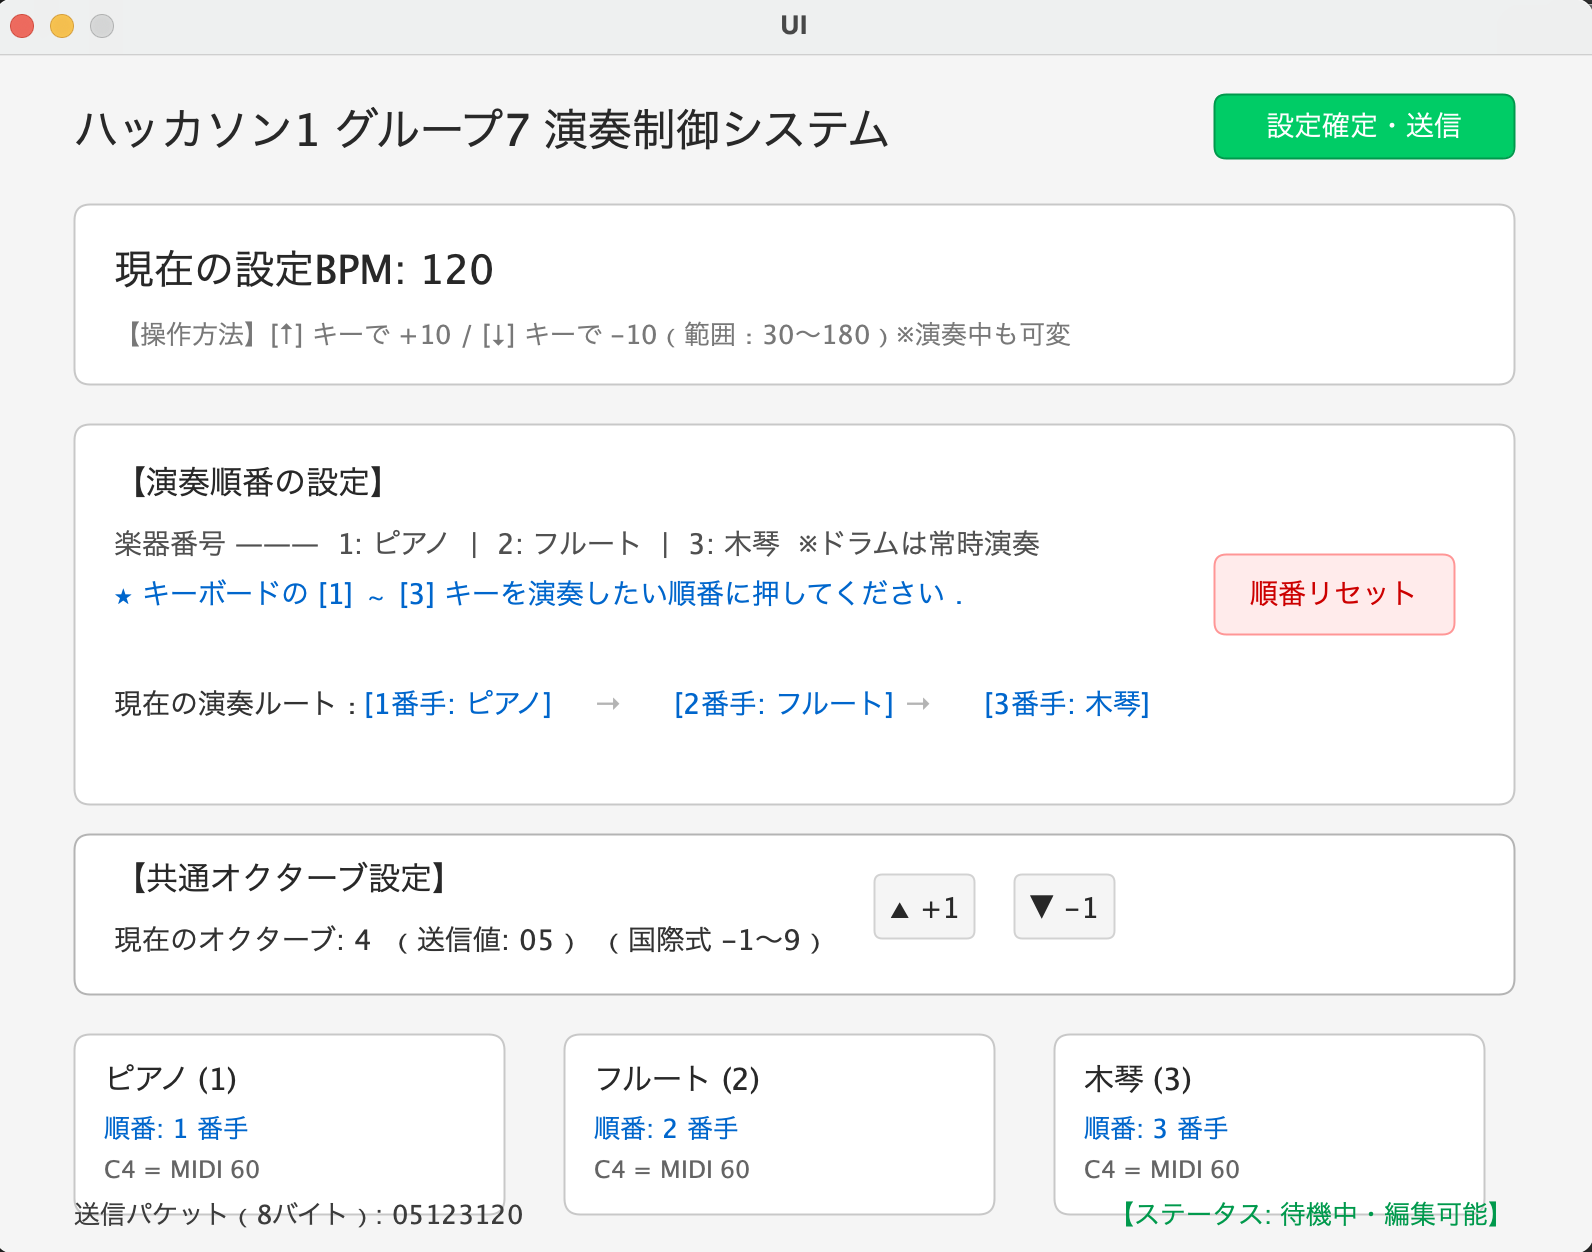
\includegraphics[width=130mm]{fig/UIgamen.png}
    }
    \caption{ProcessingのUI画面のプロトタイプ}
    \label{fig:1-5}
\end{figure}


図\ref{fig:1-5}に本システムの実際のUI画面のプロトタイプ，表\ref{tab:1-4}にUI画面上の主要な操作要素と，それぞれの操作方法および演奏中の挙動を示す．
本システムのUI画面は，BPM設定エリア，演奏順番設定エリア，共通オクターブ設定エリアの3つの操作領域と，画面右上に配置した設定確定・送信ボタンから構成される．各操作領域は，現在演奏中であるかどうかに応じて編集可否が切り替わり，ロック中は背景色を淡いグレーに変化させるとともに，該当ボタンを非活性表示にすることで，操作可能な項目を視覚的に明示している．
BPM設定エリアでは，キーボードの[$\uparrow$]キーを押すたびにBPMを$10$加算し，[$\downarrow$]キーを押すたびに$10$減算する．BPMは$30$から$180$の範囲に制限されており，この範囲を超える入力は無視される．BPMのみは演奏中であっても変更を許可しており，テンポを動的に調整できる設計としている．
演奏順番設定エリアでは，楽器番号に対応するキー（[1]：ピアノ，[2]：フルート，[3]：木琴）を押した順に演奏順を確定する．ドラムは演奏開始から常時演奏されるため，演奏順設定の対象から除外している．設定した順番は画面中央に「1番手」「2番手」「3番手」の形式で表示され，未選択の楽器は「未選択」と表示される．また，画面右側に配置した順番リセットボタン（クリック操作）を押すことで，演奏順番の選択状態を初期化できる．演奏中はこの操作領域全体がロックされ，キー入力を受け付けないとともに，リセットボタンの表示も「ロック中」に変化する．
共通オクターブ設定エリアでは，画面下部に配置した[$\blacktriangle$]ボタンおよび[$\blacktriangledown$]ボタンのクリック操作によってオクターブを1ずつ変更する．オクターブは国際式表記で$-1$から$9$の範囲とし，上限・下限を超える操作は無視される．演奏中はオクターブの加減ボタンが非活性表示となり，変更できない状態になる．

\begin{table}[H]
    \centering
    \caption{UI画面における主要操作要素と挙動}
    \label{tab:1-4}
    \small
    \renewcommand{\arraystretch}{1.3}
    \newcolumntype{M}[1]{>{\centering\arraybackslash}m{#1}}
    \newcolumntype{Y}{>{\centering\arraybackslash}X}
    \begin{tabularx}{\textwidth}{|M{3.2cm}|M{4.0cm}|Y|}
        \hline
        \textbf{UI要素} & \textbf{操作方法} & \textbf{演奏中の挙動} \\ \hline

        設定確定・送信ボタン &
        クリックにより設定をパケット化してMasterへ送信する &
        常に有効．初回は8バイトの初期パケット，2回目以降はBPM3バイトの差分パケットを送信する
        \\ \hline

        BPM設定 &
        [$\uparrow$]キーで$+10$，[$\downarrow$]キーで$-10$（範囲：$30$〜$180$） &
        演奏中も変更可能
        \\ \hline

        演奏順番設定 &
        [1]〜[3]キーを演奏したい順に押下し，ピアノ・フルート・木琴の演奏順を確定する &
        ロックされ入力を受け付けない
        \\ \hline

        順番リセットボタン &
        クリックにより演奏順番の選択状態を初期化する &
        ボタン表示が「ロック中」に変化し操作不可となる
        \\ \hline

        オクターブ[$\blacktriangle$]ボタン &
        クリックでオクターブを$+1$する（上限$9$） &
        非活性表示となり操作不可となる
        \\ \hline

        オクターブ[$\blacktriangledown$]ボタン &
        クリックでオクターブを$-1$する（下限$-1$） &
        非活性表示となり操作不可となる
        \\ \hline

    \end{tabularx}
\end{table}

\newpage

\subsubsection{Masterへのシリアル送信処理}

\begin{wrapfigure}{r}{0.45\textwidth}
    \vspace{-2em}
    \centering
    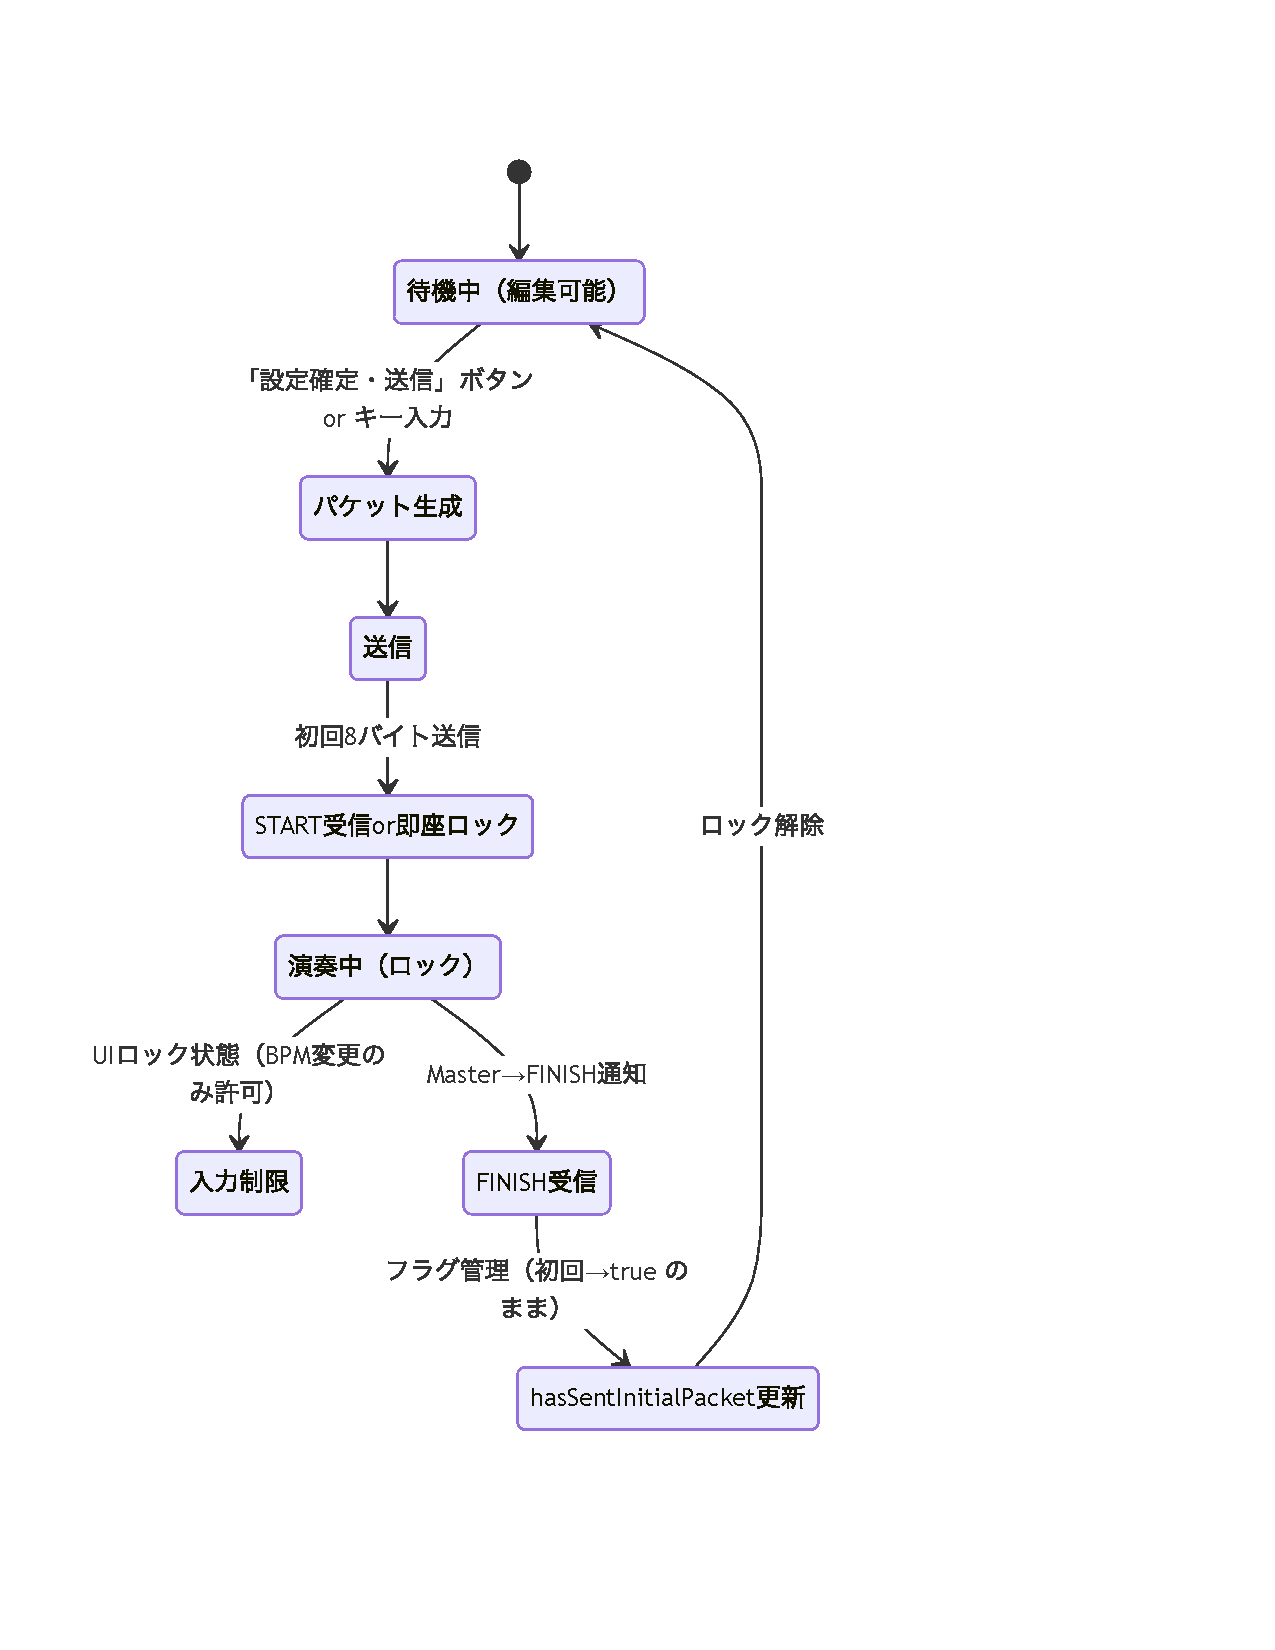
\includegraphics[width=\linewidth]{fig/ProcessingFro.pdf}
    \caption{ProcessingからMasterへの送信の状態遷移図}
    \label{fig:1-6}
\end{wrapfigure}

図\ref{fig:1-6}に，ProcessingからMasterへの送信処理における状態遷移を示す．Processing側では，待機中の状態においてBPM，演奏順，オクターブの各設定を受け付け，設定確定・送信操作が行われた時点でパケット生成処理へ遷移する．オクターブは$-1$〜$9$の範囲で入力し，送信時には$00$〜$10$の2桁固定長文字列に変換する．演奏順は楽器1〜3に対応するキー入力をもとに3桁の文字列として保持し，BPMは$30$〜$180$の範囲で3桁固定長の値として扱う．これらの値はオクターブ2桁・演奏順3桁・BPM3桁の順に連結し，Masterへ送信可能な固定長の文字列形式に整形する．
送信処理では，初回送信時と2回目以降で通信内容を切り替える．初回送信では，オクターブ，演奏順，BPMを含む8バイトの初回設定パケットに改行を付加して送信する．一方，2回目以降はBPMのみを3バイトの差分パケットとして送信し，演奏中の通信負荷を抑制する．この分岐は，初回の設定送信が完了したかどうかを内部で記憶しておくことで管理する．
また，Processing側ではMasterからの応答をシリアル受信イベントとして受け取り，状態に応じてUIロック制御を行う．Masterから演奏開始の通知（START）を受信した場合は演奏中のロック状態へ移行し，演奏順およびオクターブの変更を禁止する．演奏終了の通知（FINISH）を受信した場合はロックを解除し，再び待機中の編集可能状態へ戻る．この制御により，演奏中の誤操作を防ぎつつ，BPMのみを動的に変更できる入力インタフェースを実現している．

\newpage

\subsubsection{クマアニメーション（BearWindow）の演出制御}

\begin{figure}[H]
    \centering
    \makebox[0pt][c]{
    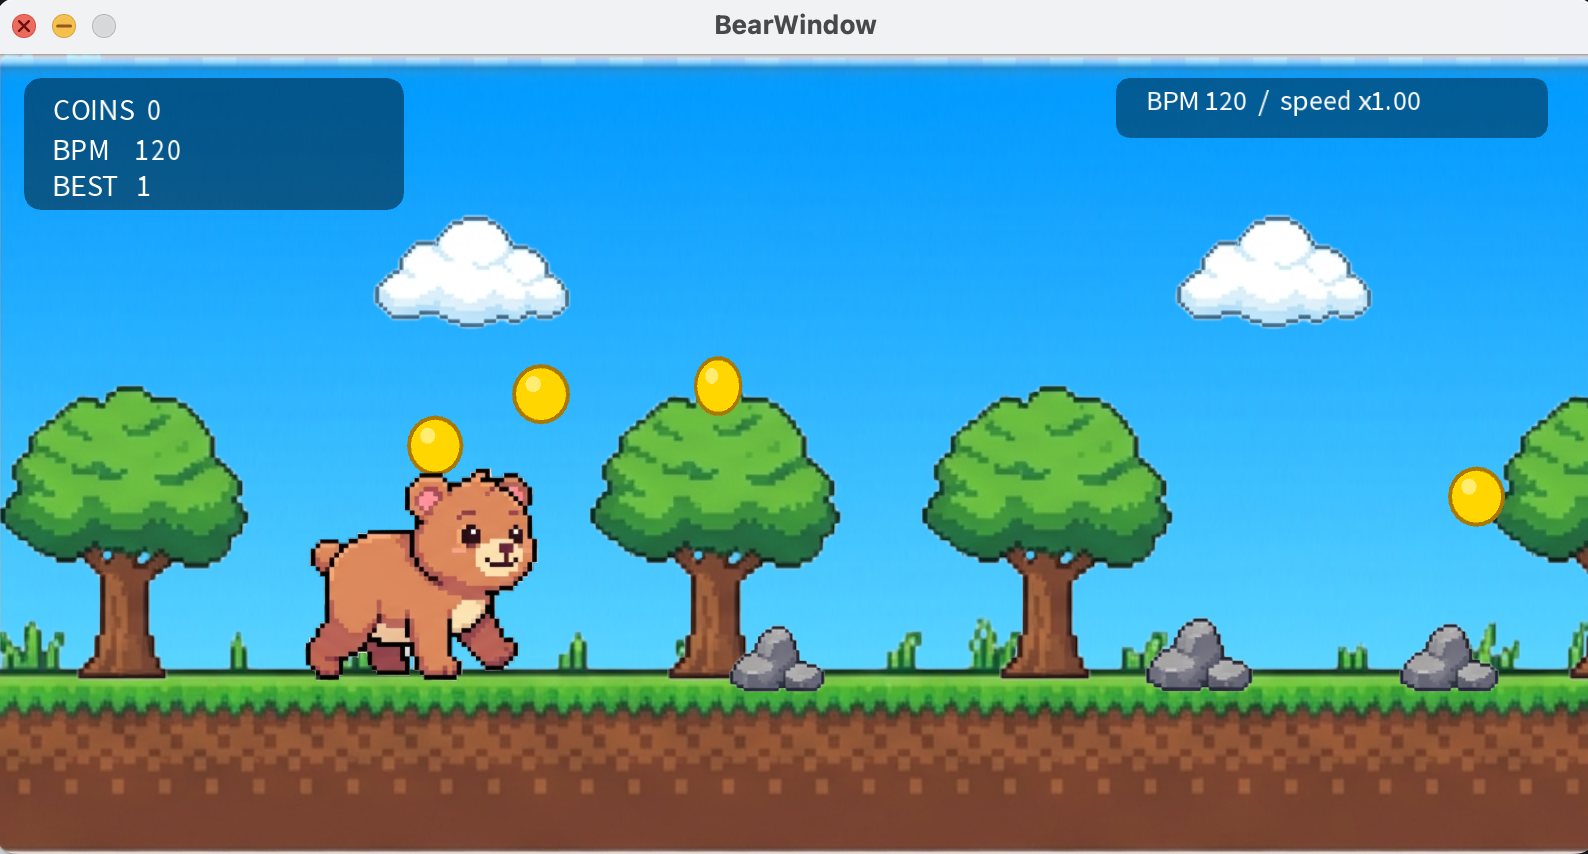
\includegraphics[width=130mm]{fig/BearWindow.png}
    }
    \caption{クマアニメーション（BearWindow）の表示画面のプロトタイプ}
    \label{fig:1-10}
\end{figure}

\begin{wrapfigure}{r}{0.45\textwidth}
    \vspace{-2em}
    \centering
    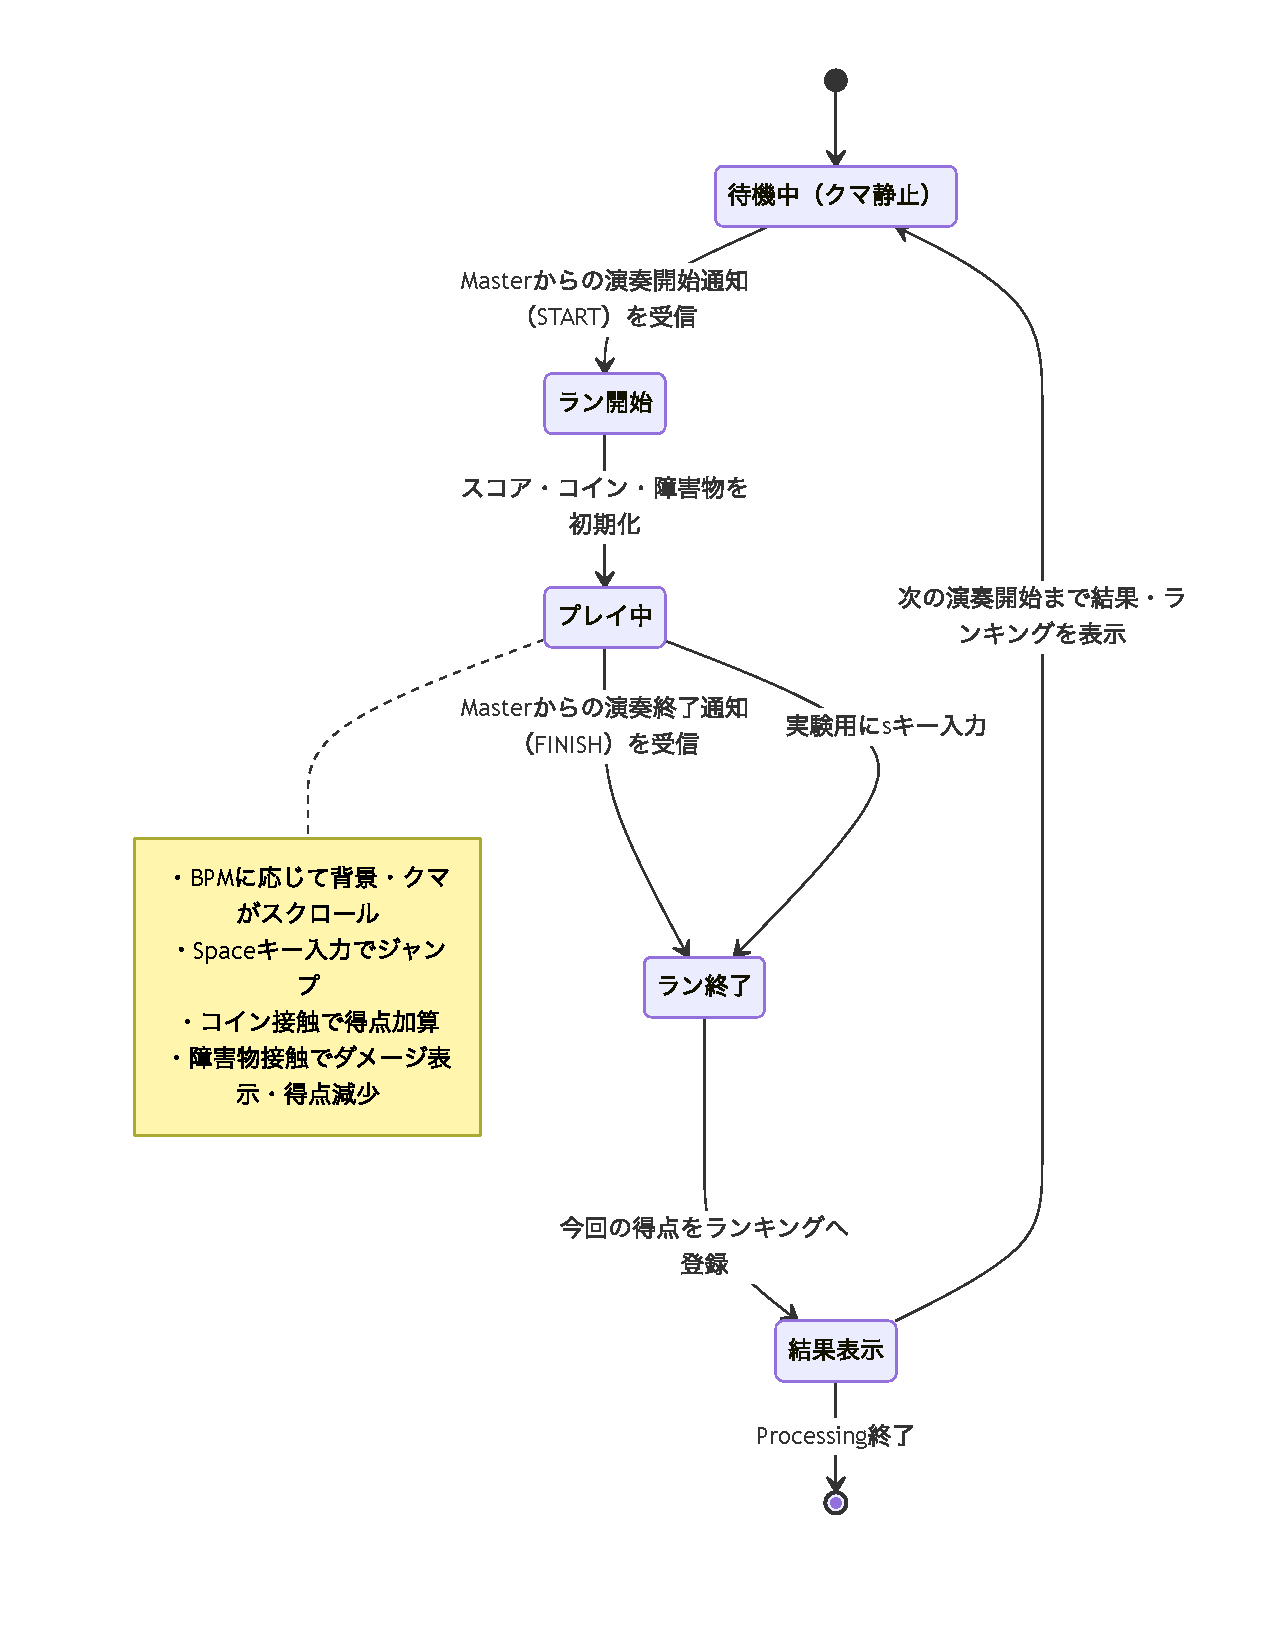
\includegraphics[width=\linewidth]{fig/BearWindowFro.pdf}
    \caption{クマアニメーションの状態遷移図}
    \label{fig:1-11}
\end{wrapfigure}

図\ref{fig:1-10}に，演奏中に表示されるクマアニメーションウィンドウの画面のプロトタイプ，図\ref{fig:1-11}にクマアニメーションの状態遷移図を示す．本ウィンドウは指揮者UIとは同一プロセス・別ウィンドウとして，指揮者UIの起動時に同時に立ち上げる構成とした．これにより，1つの操作（演奏開始）に対して，指揮者UI画面とクマアニメーション画面という2つの表示が独立して並行に動作する．両者の連携は毎フレーム指揮者UI側から現在のBPMと演奏中かどうかの状態をクマアニメーション側へ渡し，クマアニメーション側はこれらの値だけを参照して描画とゲーム進行を行う．逆方向（クマアニメーション側から指揮者UI側）への影響は，ランの結果（獲得コインとランキング）の通知のみに限定し，システム全体の制御がクマアニメーションの都合で乱れないようにしている．
描画する画像（クマの歩行2種・ジャンプ・ダメージ，および空・地面・雲2種・木2種・石）はすべてドット絵のPNGとして用意した．これらの画像は指揮者UI側でまとめて読み込んだうえでクマアニメーション側に渡し，クマアニメーション側では画像の読込み処理を行わない方針とした．これは，クマアニメーション側のウィンドウ内で直接画像を読み込むと，実行環境によっては画像ファイルの参照先を正しく認識できず，読込みに失敗する場合があるためであり，読込み処理を1か所に集約することで，どの環境でも安定して起動できるようにするための工夫である．
クマアニメーション内の処理は毎フレームの状態更新と描画の2段階に分けて実装した．状態更新では現在のBPMに応じてスクロール速度を決定し，雲・木・地面・コイン・障害物の位置を進める．スクロール速度はBPMに比例して大きくなるため演奏のテンポが速いほどクマの歩行アニメーションおよび背景の流れが速くなり，テンポ感を視覚的に把握できる．地面の画像は横方向に連続して並べ，画面の左端まで流れた分を右端へ循環させることで継ぎ目を視認させずに無限スクロールしているように見せている．
操作はキーボードの[Space]キーのみであり演奏中に[Space]キーを押すとクマがジャンプする．ジャンプは空中にいる間と接地している間で見た目を切り替え，重力を模した動きで自然に落下して着地する．クマの見た目は歩行・ジャンプ・ダメージの3状態を毎フレーム判定して切り替え，歩行中はテンポに合わせて2種類の歩行画像を交互に表示する．障害物に接触した直後は一定時間ダメージの見た目に変化させ連続してダメージを受けないよう短時間の無敵時間を設けている．
当たり判定は画面に表示する画像の見た目の大きさとは別に，クマ・コイン・障害物それぞれに専用の判定領域を設ける方式とした．クマの判定領域は画像のおおよその中心に置いた円形とし，コインとの当たり判定は距離による判定，障害物との当たり判定は円と四角形の重なり判定によって行う．この方式により見た目の画像サイズを後から調整しても当たり判定の挙動に影響を与えずに済む．コインに触れると獲得コイン数が加算され，障害物に触れると獲得コイン数が一定数減算される．
演奏が開始されるとクマアニメーション側はその変化を検知して今回分の得点集計（ラン）を自動的に開始する．演奏が終了すると，指揮者UI側からクマアニメーション側へ終了が通知され，当該ランの結果がランキングに登録される．指揮者UI側はクマアニメーション側に結果があるかどうかを確認し，結果がある場合は獲得コインとランキングを指揮者UI画面上にも表示する．

\newpage

\section{担当箇所の詳細設計}
\if0
\subsection{ハードウェア設計}
\subsubsection{回路図とI2Cの原理}
%回路図，部品表（ピン配置含めて），遮光対策（環境光）
図\ref{fig:1-8}に本システムの光同期機能を実現するために必要な回路図，表\ref{tab:1-4a}，表\ref{tab:1-5}に本システムで使用する部品表を示す．マスター機1台とスレーブ機4台のArduino Uno R4 WiFiを使用し，主I2Cバスは A4（SDA），A5（SCL）に割り当てられており，USB-Cによる給電およびシリアル通信にも対応している\cite{ref:1-4}．また，受光部にはNJL7502Lのフォトトランジスタを用い，赤外LEDとフォトトランジスタを組み合わせて光信号を検出する．本システムの通信はI2C（Inter-Integrated Circuit）を採用している．I2Cはクロック信号SCLとデータ信号SDAの2本で通信を行う同期式シリアル通信であり，信号線がオープンドレイン構成であるため，HIGHレベルを成立させるには外部プルアップ抵抗が必要である．また，I2Cではcontroller（マスタ）とtarget（スレーブ）の役割を分けて通信を行う．このため，本システムのように複数のArduinoを1つのバスで接続する構成に適している\cite{ref:1-5}．

\begin{figure}[H]
    \centering
    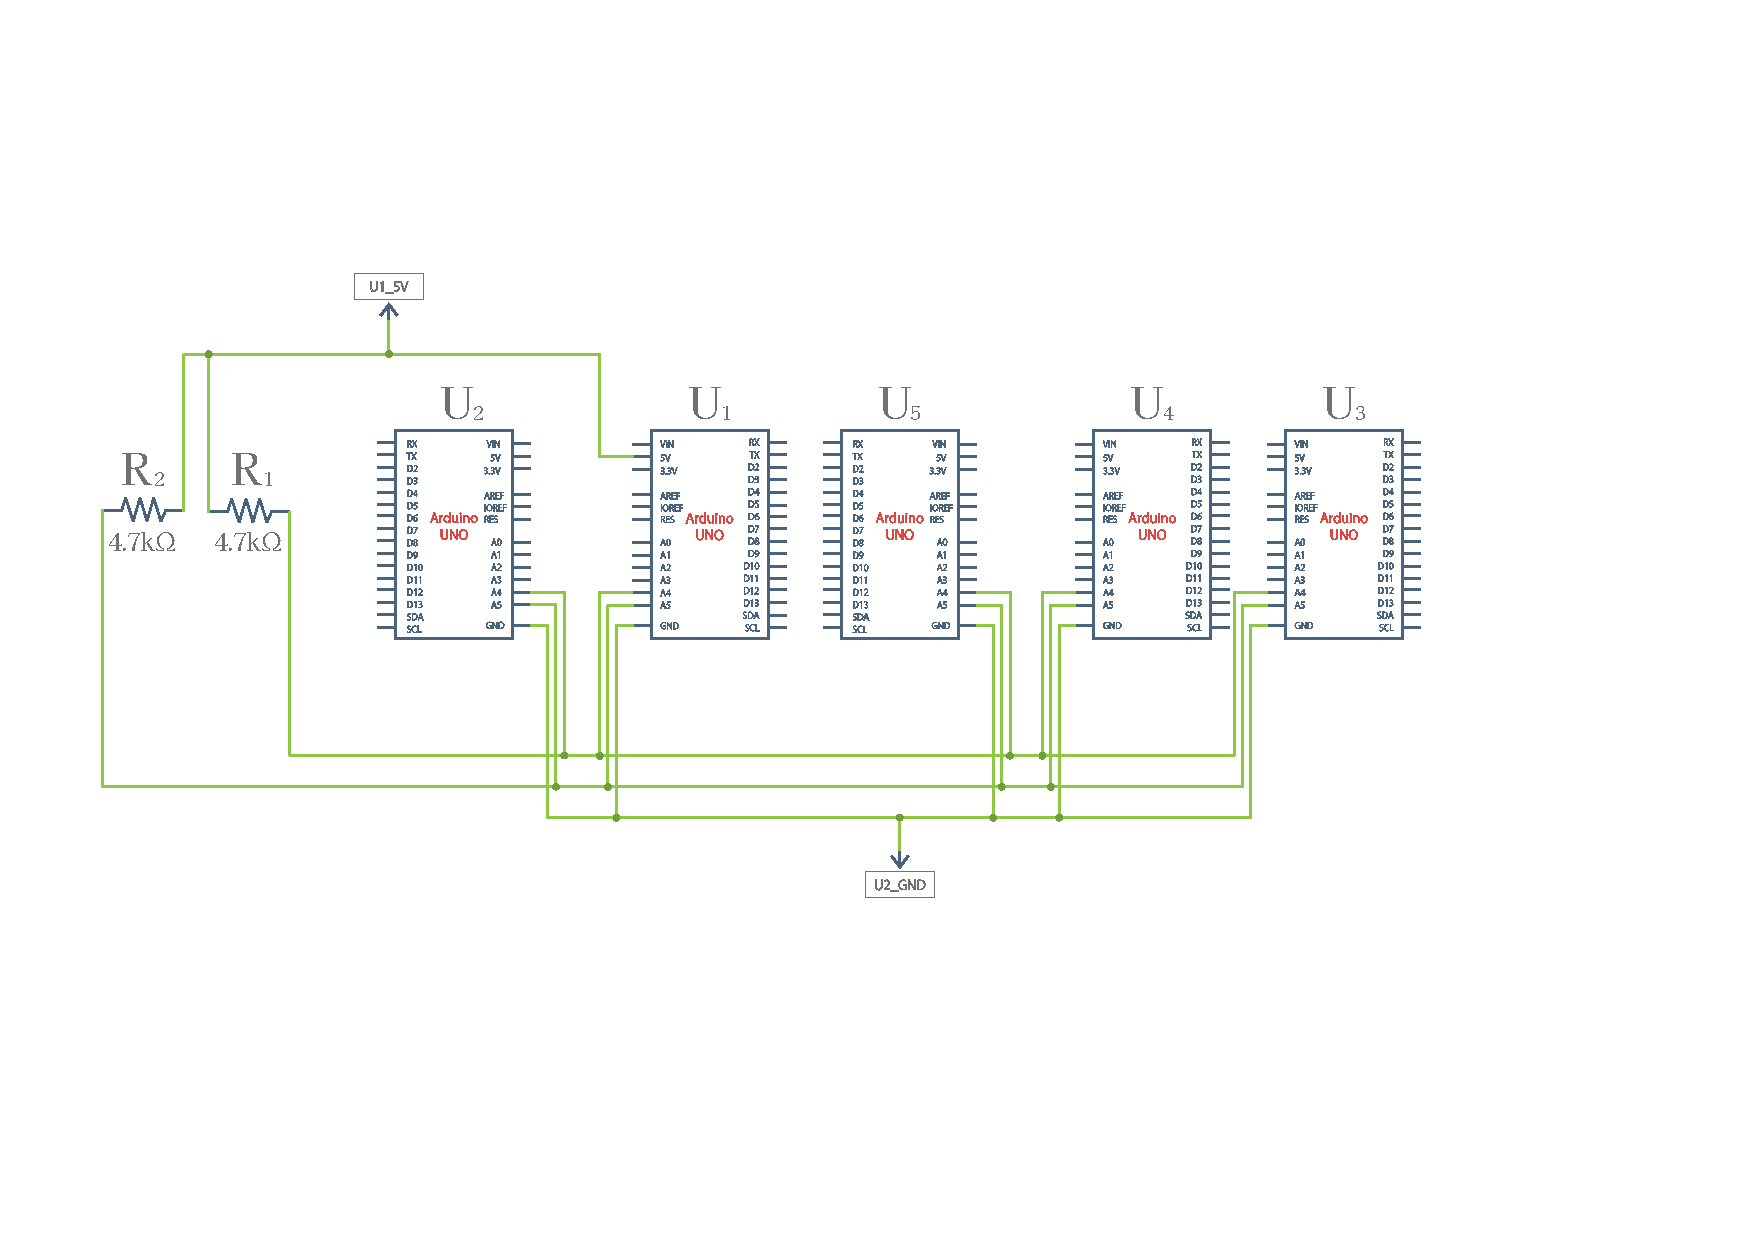
\includegraphics[width=0.95\textwidth]{fig/HCK01_kairo.pdf}
    \caption{本Arduinoオーケストラの回路図}
    \label{fig:1-8}
\end{figure}

\begin{table}[H]
  \centering
  \caption{部品表：電子部品}
  \label{tab:1-4a}
  \small
  \renewcommand{\arraystretch}{1.2}
  \newcolumntype{M}[1]{>{\centering\arraybackslash}m{#1}}
  \newcolumntype{Y}{>{\centering\arraybackslash}X}
  \begin{tabularx}{\textwidth}{|M{3.0cm}|M{2.5cm}|M{1.2cm}|Y|}
    \hline
    \textbf{部品名} & \textbf{型番} & \textbf{個数} & \textbf{用途} 
    \\ \hline
    SDAプルアップ抵抗 & 4.7k$\Omega$ & 1 &
    I2C通信のSDA線をHIGHレベルへ保持する．
     \\ \hline
    SCLプルアップ抵抗 & 4.7k$\Omega$ & 1 &
    I2C通信のSCL線をHIGHレベルへ保持する．
     \\ \hline
    炭素皮膜抵抗 & 220$\Omega$ & 1 &
    LEDの電流制限抵抗として用いる． 
    \\ \hline
    炭素皮膜抵抗 & 10k$\Omega$ & 4 &
    フォトトランジスタ受光回路のプルアップ抵抗として用いる．
     \\ \hline
    フォトトランジスタ & NJL7502L & 4 &
    LED光を受信するための光センサとして用いる．
     \\ \hline
    赤外線LED & ーー & 1 &
    同期信号送信用の光源として用いる． 
    \\ \hline
    遮光装置 & ーー & 1式 &
    外光の影響を抑え，受光値を安定化させる．
     \\ \hline
    ブレッドボード & 165401020E & 必要数 &
    回路の仮組みおよび配線整理に用いる．
     \\ \hline
    ジャンパワイヤ & 165012000E & 1式 &
    各部品間の接続に用いる． 
    \\ \hline
    USBケーブル & ーー & 5 &
    Arduinoの給電およびシリアル通信に用いる．
     \\ \hline
    USBハブ & ーー & 1 &
    複数ArduinoをPCへ同時接続するために用いる．
     \\ \hline
     \end{tabularx}
\end{table}

\begin{table}[H]
  \centering
  \caption{部品表：制御用マイコン}
  \label{tab:1-5}
  \small
  \setlength{\tabcolsep}{4pt}
  \renewcommand{\arraystretch}{1.4}
  \newcolumntype{M}[1]{>{\centering\arraybackslash}m{#1}}
  \newcolumntype{Y}{>{\centering\arraybackslash}X}
  \begin{tabularx}{\textwidth}{|M{1.5cm}|M{1.5cm}|M{1.5cm}|M{4.5cm}|Y|}
    \hline
    \textbf{識別名} &
    \textbf{役割} &
    \textbf{使用ピン} &
    \textbf{接続先} &
    \textbf{主な用途} \\ \hline

    U1 &
    同期制御マスター機 &
    A4(SDA)，A5(SCL)，D2，USB-C &
    SDA/SCLバス，赤外線LED，PC &
    BPM情報をProcessingから受信し，
    I2C通信およびLED光パルスを用いて
    各スレーブ機へ同期信号とBPMを送信する．
    \\ \hline

    U2 &
    ピアノ制御スレーブ機 &
    A4(SDA)，A5(SCL)，D3，USB-C &
    SDA/SCLバス，NJL7502L，PC &
    ピアノ楽譜データの保持，
    光同期検知，Processingへの演奏情報送信を行う．
    \\ \hline

    U3 &
    木琴制御スレーブ機 &
    A4(SDA)，A5(SCL)，D3，USB-C &
    SDA/SCLバス，NJL7502L，PC &
    木琴楽譜データの保持，
    光同期検知，Processingへの演奏情報送信を行う．
    \\ \hline

    U4 &
    フルート制御スレーブ機 &
    A4(SDA)，A5(SCL)，D3，USB-C &
    SDA/SCLバス，NJL7502L，PC &
    フルート楽譜データの保持，
    光同期検知，Processingへの演奏情報送信を行う．
    \\ \hline

    U5 &
    ドラム制御スレーブ機 &
    A4(SDA)，A5(SCL)，D3，USB-C &
    SDA/SCLバス，NJL7502L，PC &
    ドラム楽譜データの保持，
    光同期検知，Processingへの演奏情報送信を行う．
    \\ \hline
  \end{tabularx}
\end{table}

\newpage

\subsubsection{抵抗値の算出}
I2Cのプルアップ抵抗値は，I2Cバスの容量と立ち上がり時間の制約から決定する．I2Cでは信号線がオープンドレイン構成であるため，SDAおよびSCLをHIGHレベルに保つにはプルアップ抵抗が必要である．また，LOW出力時には各デバイスが許容するシンク電流の範囲内に収める必要がある．このとき，プルアップ抵抗値の下限$R_{\mathrm{p(min)}}$は式\ref{eq:1-2}で表される．
\begin{equation}
    R_{\mathrm{p(min)}} = \frac{V_{\mathrm{DD}} - V_{\mathrm{OL(max)}}}{I_{\mathrm{OL}}}
    \label{eq:1-2}
\end{equation}
ここで，$V_{\mathrm{DD}}$は電源電圧，$V_{\mathrm{OL(max)}}$はLOWレベル出力電圧の最大値，$I_{\mathrm{OL}}$はLOWレベル出力時にデバイスに流れ込む引き込み電流（シンク電流）である．式\ref{eq:1-2}に，本システムの設計値である$V_{\mathrm{DD}} = 5.0$ V，$V_{\mathrm{OL(max)}} = 0.4$ V，$I_{\mathrm{OL}} = 3$ mAを代入すると，
\begin{equation}
    R_{\mathrm{p(min)}} = \frac{5.0 - 0.4}{0.003} \approx 1.53 \ \mathrm{k}\Omega
    \label{eq:1-3}
\end{equation}
となる．一方で，抵抗値が大きすぎると信号の立ち上がりが遅くなり，I2Cの仕様を満たせなくなる．立ち上がり時間は，バスの総負荷容量$C_{\mathrm{b}}$とプルアップ抵抗値$R_{\mathrm{p}}$の積に依存する．I2Cの標準モード（Standard-mode）における最大立ち上がり時間$t_{\mathrm{r}}$の規定に基づくと，抵抗値の上限$R_{\mathrm{p(max)}}$は式\ref{eq:1-4}で求められる\cite{ref:1-5}．
\begin{equation}
    R_{\mathrm{p(max)}} = \frac{t_{\mathrm{r}}}{0.8473 \times C_{\mathrm{b}}}
    \label{eq:1-4}
\end{equation}
ここで，$t_{\mathrm{r}}$は最大立ち上がり時間（Standard-modeでは1000 ns），$C_{\mathrm{b}}$はバスの総負荷容量である．本システムのように5台のArduinoを接続し，ジャンパワイヤによる配線を行う場合，$C_{\mathrm{b}}$を約100 pFと仮定すると，$R_{\mathrm{p(max)}}$は約11.8 k$\Omega$となる．したがって，プルアップ抵抗値は$1.53 \ \mathrm{k}\Omega \leq R_{\mathrm{p}} \leq 11.8 \ \mathrm{k}\Omega$の範囲で選定する必要がある．本システムでは，実用上の安定性と汎用性を考慮し，一般的にも広く用いられている4.7 k$\Omega$を採用した．
次に，LEDの電流制限抵抗は，電源電圧，順方向電圧降下，および順方向電流の関係から決定する．電流制限抵抗$R$を算出する式を式\ref{eq:1-5}に示す．
\begin{equation}
    R = \frac{V_{\mathrm{CC}} - V_{\mathrm{F}}}{I_{\mathrm{F}}}
    \label{eq:1-5}
\end{equation}
ここで，$V_{\mathrm{CC}}$は電源電圧，$V_{\mathrm{F}}$はLEDの順方向電圧降下，$I_{\mathrm{F}}$はLEDに流す順方向電流を示す．式\ref{eq:1-5}に，$V_{\mathrm{CC}} = 5.0$ V，$V_{\mathrm{F}} = 2.0$ V，$I_{\mathrm{F}} = 15$ mAを代入すると，
\begin{equation}
    R = \frac{5.0 - 2.0}{0.015} = 200 \ \Omega
    \label{eq:1-6}
\end{equation}
となる．そのため，入手性の高い標準値の中から220 $\Omega$を採用した．
最後に，フォトトランジスタNJL7502Lの受光回路においては，光電流がLEDとの距離，角度，および周囲光の強さなどの環境要因に大きく依存するため，理論式のみで抵抗値を一意に決定することは難しい．このため，本システムでは基準値として10 k$\Omega$を選定し，実装時にArduinoのAnalogReadを用いて受光電圧を測定しながら，実測ベースで逐次調整する方針とした．
\fi

\subsection{ソフトウェア設計}
%全体の処理フローチャート，関数表，変数表，環境光のノイズ除去と閾値の設定について触れる

\subsubsection{全体の処理フロー}
システム全体のフローチャートを図\ref{fig:1-9}，図\ref{fig:1-10}に示す．本処理は，Processingの起動時に\texttt{setup()}が実行され，シリアルポートを9600bpsで初期化するところから開始する．接続に成功した場合は\texttt{isSerialConnected}を\texttt{true}に設定し，失敗した場合はシミュレーションモードとして\texttt{isSerialConnected=false}のままUI初期化を完了する．続いて\texttt{setup()}内では，クマアニメーション用の別ウィンドウ\texttt{BearWindow}を生成し，クマおよび背景・地形・障害物に用いる11種類のドット絵画像をメインスケッチ側で\texttt{loadImage()}した上で\texttt{bearWin}へ受け渡し，最後に\texttt{PApplet.runSketch()}によってBearWindowを起動する．これにより，指揮者UIとクマアニメーションは同一プロセス内の2枚の独立したウィンドウとして並行に動作する構成となる．初期化完了後は\texttt{draw()}によるメインループに入り，UIの描画とユーザー操作の受付を毎フレーム繰り返すとともに，現在のBPMと演奏中フラグ\texttt{isPlaying}を\texttt{bearWin.bearBpm}，\texttt{bearWin.bearPlaying}へ書き込み，BearWindow側の描画内容と同期する．
ユーザー操作は，BPM変更，演奏順設定，オクターブ変更，送信，ジャンプの5系統に分岐する．BPMは↑／↓キー入力により30〜180の範囲で更新される．演奏順は1〜3キー入力により設定されるが，\texttt{isPlaying=true}の間は変更できず，待機中のみ\texttt{playOrder[]}へ反映される．オクターブもボタンクリックによって-1〜9の範囲で更新されるが，同様に演奏中は操作を無効化する．スペースキーが押下されると，押し続け判定用フラグ\texttt{bearJumpKeyHeld}によって1回の押下につき1度だけ\texttt{bearWin.triggerJump()}が呼び出され，BearWindow側のクマがジャンプする．送信ボタンが押されると\texttt{sendParametersToMaster()}が呼び出され，Masterへの送信処理へ遷移する．
送信処理では，\texttt{hasSentInitialPacket}の値によって初回送信と2回目以降の送信を切り替える．初回送信では，オクターブ2桁，演奏順3桁，BPM3桁を連結した初回パケットを\texttt{buildPacket()}で生成し，シリアル接続時はMasterへ送信する．送信完了後は\texttt{hasSentInitialPacket}を\texttt{true}に更新し，\texttt{isPlaying=true}としてUIをロックする．この\texttt{isPlaying}の変化はBearWindow側へ同期され，BearWindowの\texttt{draw()}が変化を検知して\texttt{startRun()}を呼び出すことで，今回のランを開始し，コイン・障害物・スコアを初期化したうえでBPMに応じたスクロール演出を開始する．2回目以降の送信はBPMのみを3桁で送信し，演奏中のテンポ変更に対応する．
また，Masterからの状態通知は\texttt{serialEvent()}で受信する．\texttt{START}または\texttt{PLAYING}を受信した場合は\texttt{isPlaying=true}を維持してロック状態を継続し，\texttt{FINISH}または\texttt{STOP}を受信した場合は\texttt{completeCurrentRun()}を呼び出して\texttt{isPlaying=false}とするとともに，BearWindow側の\texttt{completeRun()}を実行してランを終了させ，獲得コインをランキングに登録する．シリアル未接続のシミュレーションモードでは，送信ボタン押下時に擬似的にロックし，sキー押下で同様に\texttt{completeCurrentRun()}を呼び出すことでランの終了を代替する．ランが終了すると，指揮者UI側では\texttt{drawRunResultPanel()}が毎フレーム\texttt{bearWin.hasResult()}を確認し，結果がある場合に獲得コインとランキングを画面上へ表示する．これにより，演奏中の設定変更を防ぎつつ，演奏終了後は再び設定入力が可能な状態へ戻るとともに，演奏のテンポに連動した視覚的な演出とその結果のフィードバックを実現している．

\begin{figure}[H]
    \centering
    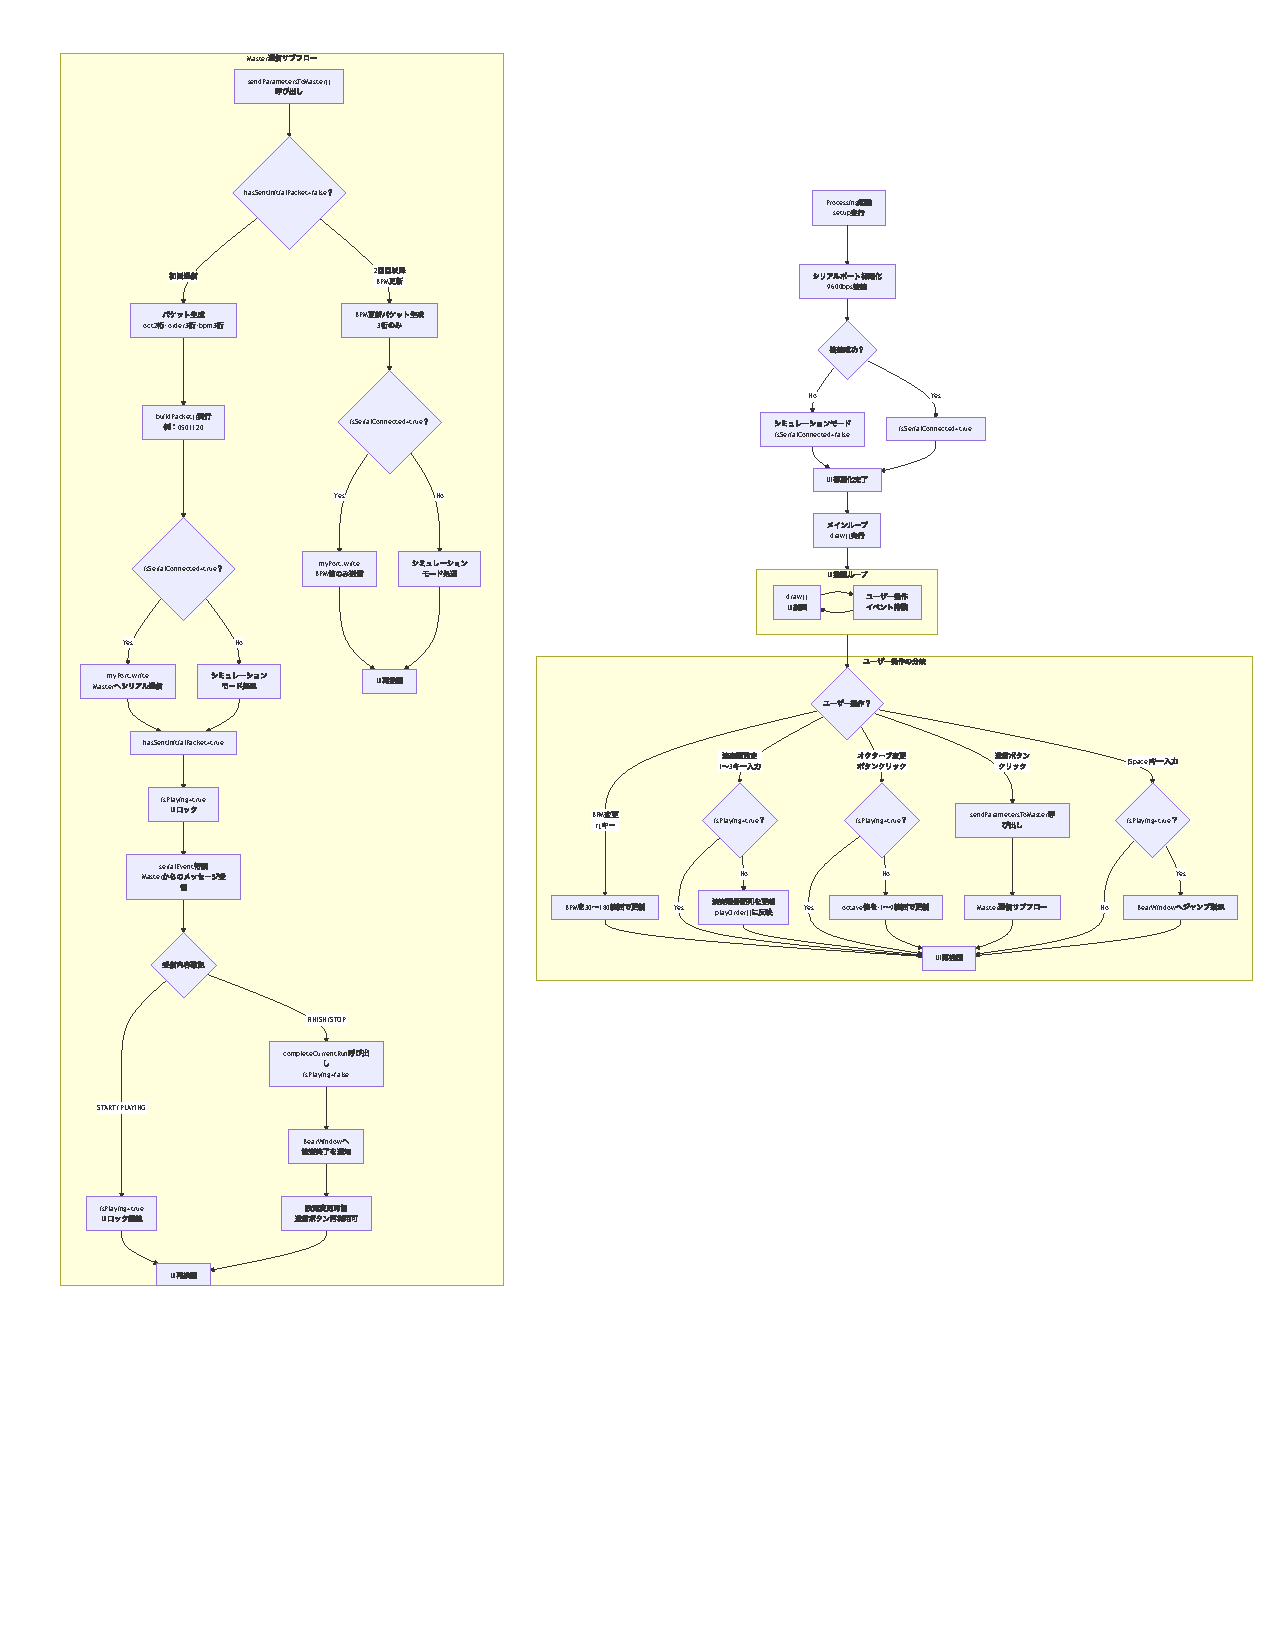
\includegraphics[width=150mm]{fig/UIzentaiFro.pdf}
    \caption{UI，Masterへの送信制御フローチャート}
    \label{fig:1-9}
\end{figure}

\begin{figure}[H]
    \centering
    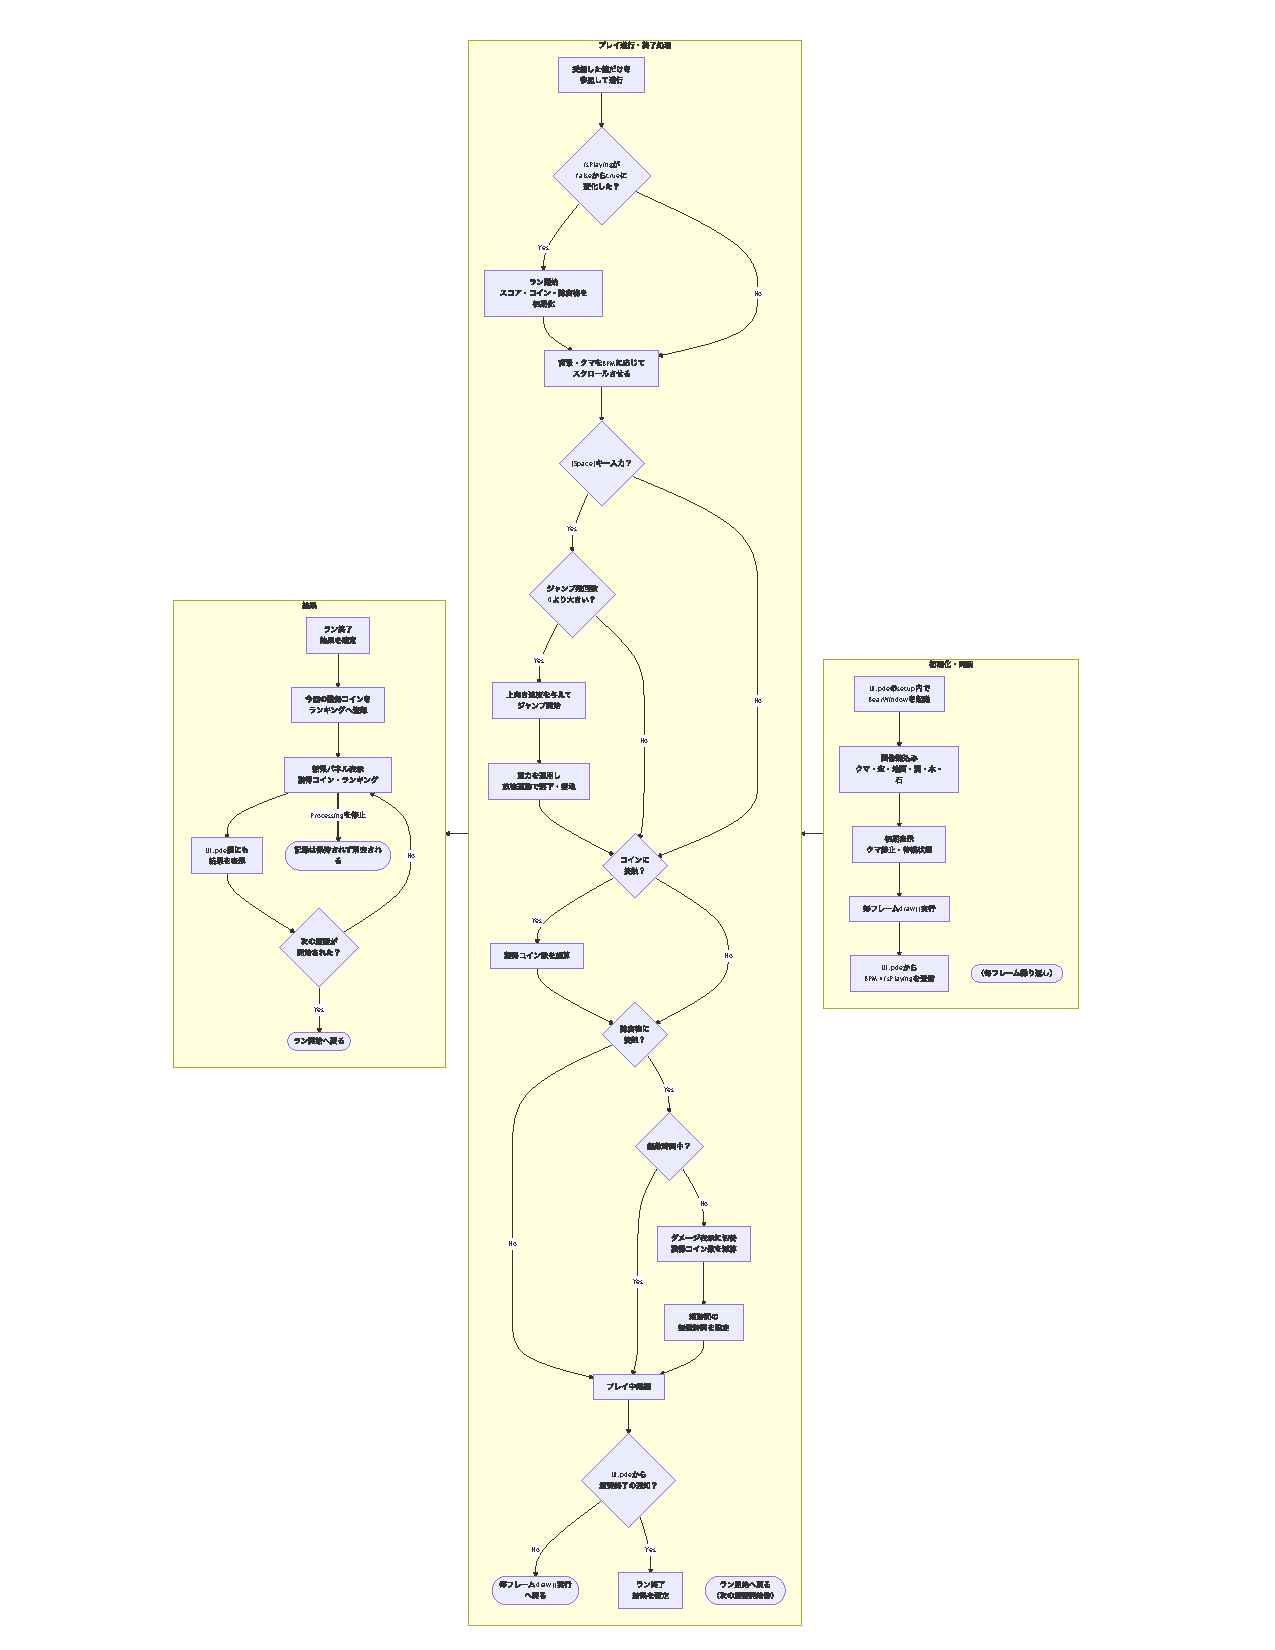
\includegraphics[width=130mm]{fig/BearWindowzentaiFro.pdf}
    \caption{クマアニメーション同期のフローチャート}
    \label{fig:1-10}
\end{figure}


\subsubsection{主要関数表}

表\ref{tab:1-6-1}に示した主要関数について，制御の流れに沿ってその役割を述べる．
UI.pdeの\texttt{setup()}では，シリアル接続の確立に続いて画像の読込みとBearWindowの起動を行う．\texttt{draw()}は毎フレーム呼び出される唯一の描画起点であり，UI各エリアの描画に加えて，\texttt{buildPacket()}による送信パケットのプレビュー表示，BearWindowへのBPM・演奏状態の同期，および\texttt{drawRunResultPanel()}による結果パネルの描画をまとめて行う．キー入力は\texttt{keyPressed()}と\texttt{keyReleased()}に分離されており，BPM変更，演奏順設定，ジャンプ発火，シミュレーション時の終了操作（sキー）をそれぞれ判定する．マウス操作は\texttt{mousePressed()}に集約され，送信ボタン，リセットボタン，オクターブ増減ボタンへのクリックをホバー判定関数\texttt{isHover()}を用いて検出する．
ランの開始と終了は，UI.pde側の\texttt{completeCurrentRun()}と，BearWindow側の\texttt{startRun()}，\texttt{completeRun()}が対になって管理する．\texttt{completeCurrentRun()}は\texttt{isPlaying}の解除とBearWindowへの終了通知を1か所に集約するための関数であり，シリアル受信時とシミュレーション時の両方から呼び出される．BearWindow内部では，\texttt{updateWorld()}が毎フレームの状態更新（スクロール，ジャンプ，コイン・障害物判定，アニメーション状態）を統括し，\texttt{draw()}が背景・地形・コイン・障害物・クマ・HUDの描画を順に呼び出す．当たり判定は\texttt{isCoinCollected()}，\texttt{isObstacleHit()}，および円と矩形の判定を行う\texttt{circleRectOverlap()}によって実装し，画像のサイズに依存しない独立した判定オブジェクトとして扱う．

\renewcommand{\arraystretch}{1.25}
\newcolumntype{M}[1]{>{\centering\arraybackslash}m{#1}}
\newcolumntype{Y}{>{\centering\arraybackslash}X}

{\small
\begin{tabularx}{\textwidth}{|M{1.6cm}|M{3.3cm}|M{2.1cm}|Y|}
    \caption{主要関数表}\label{tab:1-6-1}\\
    \hline
    \textbf{戻り値} & \textbf{関数名} & \textbf{引数} & \textbf{役割} \\ \hline
    \endfirsthead
    \multicolumn{4}{c}{\tablename\ \thetable\ （続き）}\\
    \hline
    \textbf{戻り値} & \textbf{関数名} & \textbf{引数} & \textbf{役割} \\ \hline
    \endhead
    \hline
    \multicolumn{4}{r}{次ページに続く}\\
    \endfoot
    \hline
    \endlastfoot

    \multicolumn{4}{|c|}{\textbf{UI.pde}} \\ \hline
    void & setup & なし & シリアル接続の確立，フォント設定，クマ画像群の読込み，BearWindowの起動を行う初期化関数． \\ \hline
    void & draw & なし & 毎フレーム呼び出され，UI各エリアの描画，BearWindowへのBPM・演奏状態の同期，結果パネルの描画をまとめて行う． \\ \hline
    void & keyPressed & なし & ↑／↓キーによるBPM変更，スペースキーによるジャンプ発火，1〜3キーによる演奏順設定，sキーによる終了操作を判定する． \\ \hline
    void & keyReleased & なし & スペースキーが離されたことを検知し，ジャンプの押し続け判定フラグを解除する． \\ \hline
    void & mousePressed & なし & 送信・リセット・オクターブ増減ボタンへのクリックを判定し，対応する処理を呼び出す． \\ \hline
    void & serialEvent & port & Masterからの受信文字列を解析し，START／PLAYING時はロック，FINISH／STOP時はランの終了処理を行う． \\ \hline
    boolean & isHover & x, y, w, h & マウス座標が指定した矩形領域内にあるかを判定する． \\ \hline
    void & resetOrder & なし & 演奏順番および選択状態を未設定の状態に初期化する． \\ \hline
    void & completeCurrentRun & message & \texttt{isPlaying}を解除し，BearWindow側の\texttt{completeRun()}を呼び出してランを終了させる． \\ \hline
    void & drawRunResultPanel & なし & BearWindowにランの結果がある場合に，獲得コインとランキングを指揮者UI画面上へ描画する． \\ \hline
    String & buildPacket & なし & オクターブ・演奏順・BPMを8バイトの固定長文字列にエンコードする． \\ \hline
    void & sendParametersToMaster & なし & 初回は8バイトの初期パケット，以降はBPMのみの3バイトパケットをMasterへ送信する． \\ \hline

    \multicolumn{4}{|c|}{\textbf{BearWindow.pde}} \\ \hline
    void & setup & なし & フレームレートの固定，各オブジェクトの初期座標および種類（雲・木）の抽選，コイン・障害物・パーティクルの初期化を行う． \\ \hline
    void & draw & なし & 毎フレーム呼び出され，\texttt{updateWorld()}による状態更新の後，背景・地形・コイン・障害物・クマ・HUDを順に描画する． \\ \hline
    void & updateWorld & なし & BPMに応じたスクロール速度の算出，雲・木・地面・ジャンプ・コイン・障害物の状態更新をまとめて行う． \\ \hline
    float & getScrollSpeed & なし & 現在のBPMと演奏中フラグから，背景・オブジェクトのスクロール速度を算出する． \\ \hline
    void & updateBearState & なし & ダメージ・ジャンプ・歩行のいずれかにクマの表示状態\texttt{bearState}を更新する． \\ \hline
    void & drawBear & x, y, angle & 現在の状態に対応するドット絵画像を選択し，足元の補正値を加味してクマを描画する． \\ \hline
    PImage & currentBearImage & angle & \texttt{bearState}と歩行位相から，表示すべきクマ画像（歩行2種／ジャンプ／ダメージ）を返す． \\ \hline
    float & bearHitCenterX & なし & クマの当たり判定円の中心のX座標を返す． \\ \hline
    float & bearHitCenterY & なし & クマの当たり判定円の中心のY座標を，ジャンプ量および足元補正値を加味して返す． \\ \hline
    void & drawGround & なし & 地面画像をオーバーラップさせながら水平方向にタイル状に描画し，継ぎ目のない無限スクロールを実現する． \\ \hline
    void & triggerJump & なし & 残りジャンプ可能回数が0より大きい場合に，初期上向き速度を与えてジャンプを発火する． \\ \hline
    void & updateJump & なし & 重力による加速度を適用し，クマのジャンプによる上下移動量を更新する． \\ \hline
    boolean & isCoinCollected & i & クマの当たり判定円と指定したコインとの距離から，収集判定を行う． \\ \hline
    boolean & isObstacleHit & i & クマの当たり判定円と指定した障害物の矩形との衝突を判定する． \\ \hline
    boolean & circleRectOverlap & cx, cy, r, rx, ry, rw, rh & 円と矩形の最近接点距離を用いて，円と矩形の衝突を判定する汎用関数． \\ \hline
    void & applyObstaclePenalty & i & 障害物接触時に獲得コインを減算し，無敵時間の設定とエフェクトの発生を行う． \\ \hline
    void & startRun & bpm & 今回のランのスコア・コイン・障害物・タイマーをすべて初期化し，ランを開始する． \\ \hline
    void & completeRun & なし & ランを終了し，獲得コインをランキング配列へ挿入する． \\ \hline
    int & insertRanking & score & 渡されたスコアをランキング配列の適切な位置へ挿入し，順位を返す． \\ \hline
    String[] & getRankingLines & なし & ランキング配列を表示用の文字列配列に整形して返す． \\ \hline
    boolean & hasResult & なし & 直前のランの結果が確定済みかどうかを返す． \\ \hline
    int & getCurrentRunScore & なし & 現在のランで獲得しているコイン数を返す． \\ \hline
\end{tabularx}
}

\subsubsection{主要変数および定数}

表\ref{tab:1-7-1}に示した主要変数および定数について，システム動作に果たす役割を述べる．
UI.pde側では，現在のテンポを保持する\texttt{bpm}，演奏順を保持する\texttt{playOrder[]}，共通オクターブを保持する\texttt{octave}が，送信パケットを構成する中核の変数である．これらは演奏中フラグ\texttt{isPlaying}の状態に応じて変更可否が切り替わり，\texttt{isPlaying}自体はMasterからのシリアル受信または\texttt{completeCurrentRun()}の呼び出しによって更新される．BearWindowとの連携は，参照を保持する\texttt{bearWin}と，スペースキーの押し続けを管理する\texttt{bearJumpKeyHeld}によって行われる．
BearWindow.pde側では，BPMに対するスクロール速度の基準となる\texttt{BASE\_BPM}，\texttt{BASE\_SPEED}と，ジャンプの物理特性を決める\texttt{GRAVITY}，\texttt{JUMP\_VELOCITY}，\texttt{MAX\_JUMPS}が描画・操作の基準値となる．クマの位置は\texttt{BEAR\_X}，\texttt{BEAR\_GROUND\_Y}を基準座標とし，画像の見た目と当たり判定の中心とのずれを\texttt{BEAR\_FOOT\_OFFSET}，\texttt{TREE\_FOOT\_OFFSET}，\texttt{OBSTACLE\_FOOT\_OFFSET}で補正する．当たり判定の半径は\texttt{BEAR\_HIT\_RADIUS}として見た目の画像サイズより小さく設定し，判定の公平性を保っている．コイン・障害物・パーティクルはそれぞれ固定長配列（\texttt{coinX[]}等，\texttt{obstacleX[]}等，\texttt{scatterX[]}等）で位置と状態を管理し，配列長は\texttt{COIN\_COUNT}，\texttt{OBSTACLE\_COUNT}，\texttt{SCATTER\_COUNT}によって定める．スコア関連では，現在のランで獲得したコイン数を\texttt{currentRunScore}，過去最高記録を\texttt{bestScore}，直近5回の記録を\texttt{rankingScores[]}に保持する．

\renewcommand{\arraystretch}{1.25}
\newcolumntype{M}[1]{>{\centering\arraybackslash}m{#1}}
\newcolumntype{Y}{>{\centering\arraybackslash}X}

{\small
\begin{tabularx}{\textwidth}{|M{1.6cm}|M{3.7cm}|M{2.9cm}|Y|}
    \caption{主要変数および定数表}\label{tab:1-7-1}\\
    \hline
    \textbf{型} & \textbf{変数名} & \textbf{初期値} & \textbf{役割} \\ \hline
    \endfirsthead
    \multicolumn{4}{c}{\tablename\ \thetable\ （続き）}\\
    \hline
    \textbf{型} & \textbf{変数名} & \textbf{初期値} & \textbf{役割} \\ \hline
    \endhead
    \hline
    \multicolumn{4}{r}{次ページに続く}\\
    \endfoot
    \hline
    \endlastfoot

    \multicolumn{4}{|c|}{\textbf{UI.pde}} \\ \hline
    int & bpm & 120 & 現在の設定BPMを保持する．30〜180の範囲で更新される． \\ \hline
    int[] & playOrder & \{0, 0, 0\} & ピアノ・フルート・木琴の演奏順（0は未設定）を保持する． \\ \hline
    int & octave & 4 & 共通オクターブ（国際式$-1$〜$9$）を保持する． \\ \hline
    boolean & isPlaying & false & 演奏中かどうかを示し，trueの間はBPM以外の変更をロックする． \\ \hline
    boolean & hasSentInitialPacket & false & 初回設定パケットを送信済みかどうかを示す． \\ \hline
    boolean & isSerialConnected & false & Masterとのシリアル接続に成功したかどうかを示す． \\ \hline
    BearWindow & bearWin & なし & クマアニメーション別ウィンドウへの参照を保持する． \\ \hline
    boolean & bearJumpKeyHeld & false & スペースキーの押し続けを判定し，ジャンプの多重発火を防ぐ． \\ \hline

    \multicolumn{4}{|c|}{\textbf{BearWindow.pde}} \\ \hline
    float & bearBpm & 120.0 & UI.pdeから同期される現在のBPMを保持する． \\ \hline
    boolean & bearPlaying & false & UI.pdeから同期される演奏中フラグを保持する． \\ \hline
    final float & BASE\_BPM & 120.0 & スクロール速度の基準となるBPM値を保持する． \\ \hline
    final float & BASE\_SPEED & 4.0 & 基準BPM時のスクロール速度を保持する． \\ \hline
    final float & GRAVITY & 0.9 & ジャンプ中にクマへ適用する重力加速度を保持する． \\ \hline
    final float & JUMP\_VELOCITY & $-14.5$ & ジャンプ発火時の初期上向き速度を保持する． \\ \hline
    final int & MAX\_JUMPS & 2 & 連続でジャンプ可能な最大回数を保持する（二段ジャンプ）． \\ \hline
    final float & BEAR\_X & 210.0 & クマの水平表示位置（画面上で固定）を保持する． \\ \hline
    final float & BEAR\_GROUND\_Y & 250.0 & クマの接地基準Y座標を保持する． \\ \hline
    final float & BEAR\_FOOT\_OFFSET & 65.0 & クマ画像の足元位置と接地基準Y座標とのずれを補正する． \\ \hline
    final float & TREE\_FOOT\_OFFSET & 35.0 & 木の画像の根元位置を地面ラインに合わせるための補正値． \\ \hline
    final float & OBSTACLE\_FOOT\_OFFSET & 40.0 & 障害物（石）の表示位置を補正する値（当たり判定には影響しない）． \\ \hline
    final float & BEAR\_HIT\_RADIUS & 30.0 & クマの当たり判定円の半径を保持する． \\ \hline
    int & bearState & BEAR\_STATE\_WALK & クマの現在の表示状態（歩行／ジャンプ／ダメージ）を保持する． \\ \hline
    float & legAngle & 0 & 歩行アニメーションの位相を保持し，BPMに応じて進行速度が変わる． \\ \hline
    float & bearJumpY & 0 & クマのジャンプによる上下方向の変位量を保持する． \\ \hline
    int & jumpsRemaining & MAX\_JUMPS & 接地までに残っているジャンプ可能回数を保持する． \\ \hline
    final int & COIN\_COUNT & 7 & 画面内に存在させるコインの個数を保持する． \\ \hline
    final int & OBSTACLE\_COUNT & 4 & 画面内に存在させる障害物の個数を保持する． \\ \hline
    int & currentRunScore & 0 & 現在のランで獲得したコイン数を保持する． \\ \hline
    int & bestScore & 0 & 起動後の最高獲得コイン数を保持する． \\ \hline
    int[] & rankingScores & \{0,0,0,0,0\} & 直近のラン結果上位5件のスコアを保持する． \\ \hline
    boolean & runFinished & false & 現在のランが終了し，結果が確定済みかどうかを示す． \\ \hline
\end{tabularx}
}

\newpage

\section{付録}
\begin{itemize}
    \item \textbf{添付資料：}
    \begin{itemize}
    	\item 回路図： 
	\begin{figure}[H]
  \centering
  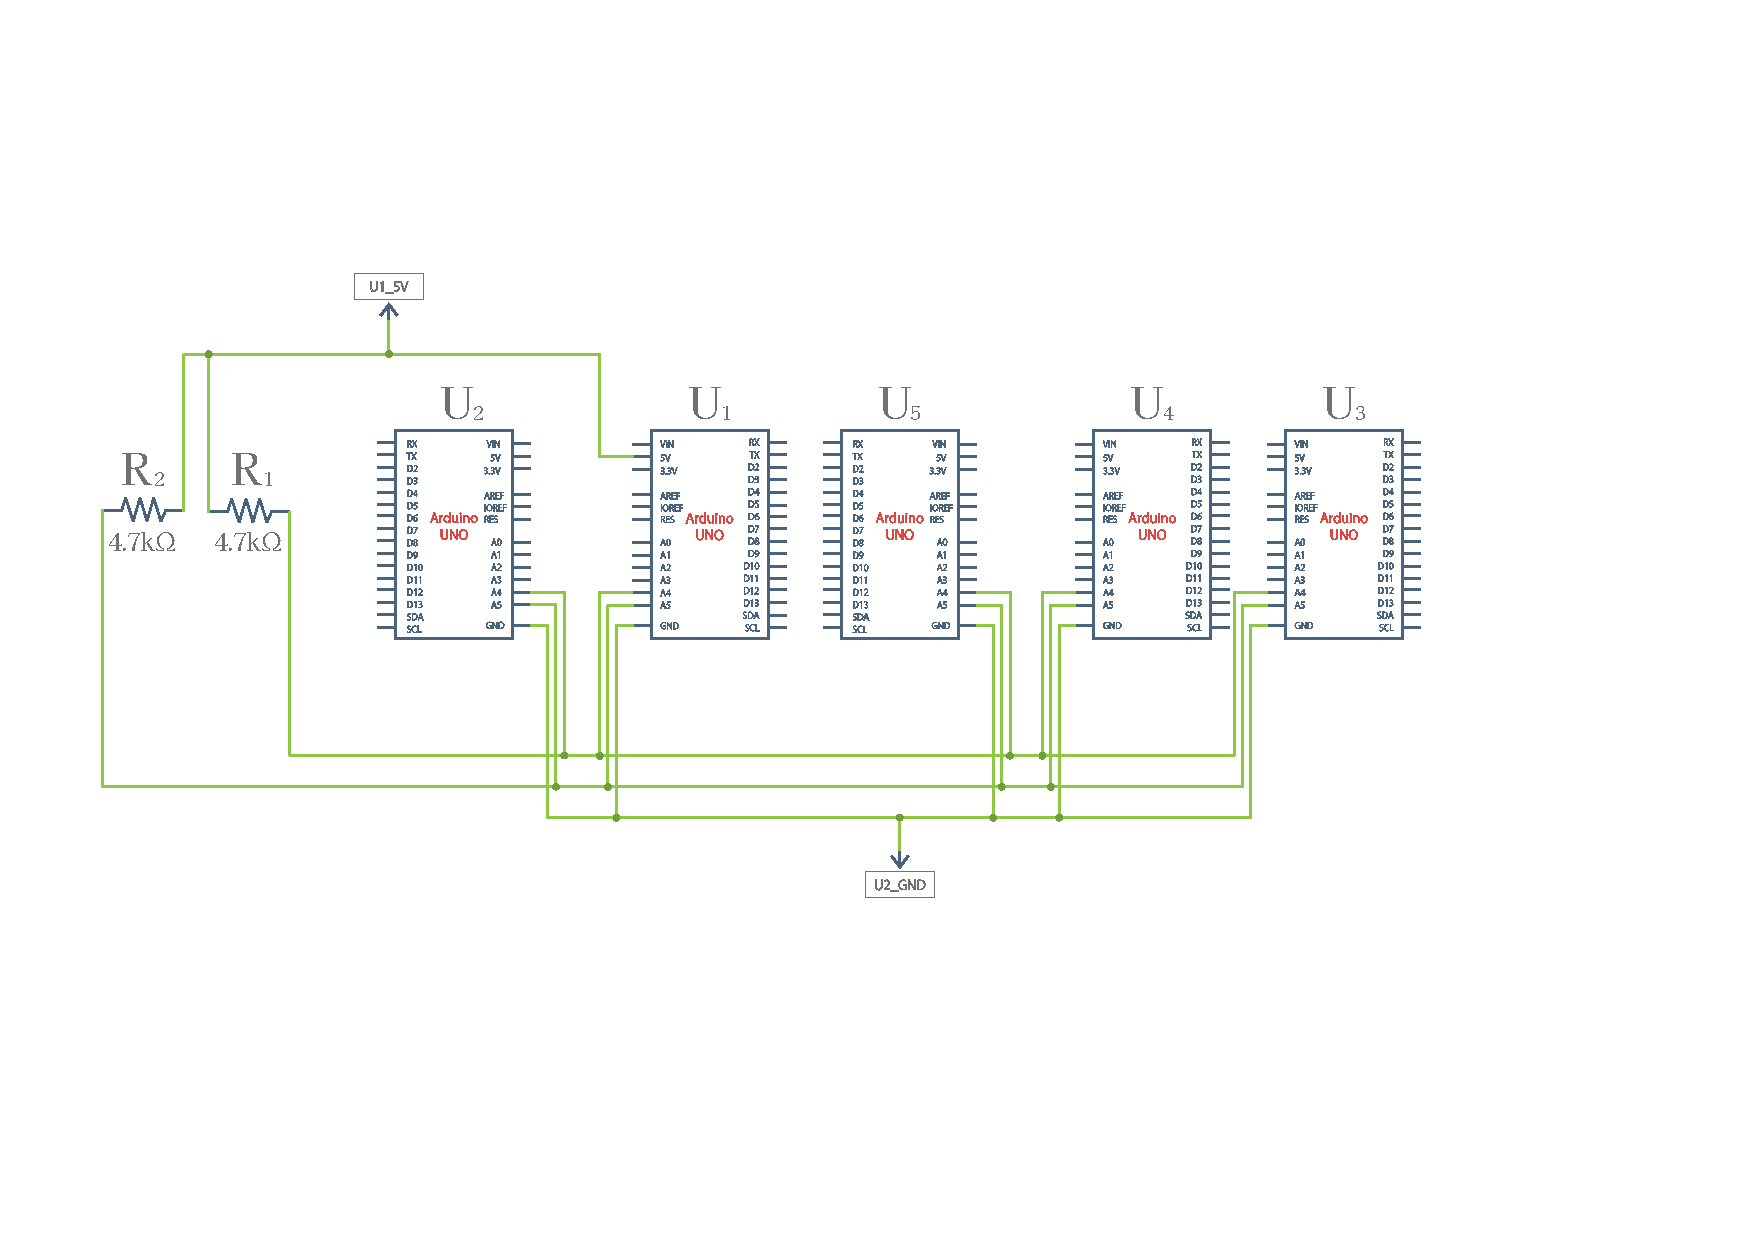
\includegraphics[width=15cm]{fig/HCK01_kairo.pdf} 
  \caption{Arduinoオーケストラの回路図}
  \label{fig:1-11}
  \end{figure}
        \item ソースコード： \\
        メインリポジトリ：\url{https://github.com/GingerAle0220/HCK01_group7}\\
        UIおよびクマさんアニメーション：\url{https://github.com/GingerAle0220/HCK01_group7/tree/main/UI_ver.3}\\
        設計書\_UI：\url{https://github.com/GingerAle0220/HCK01_group7/tree/main/\%E8\%A8\%AD\%E8\%A8\%88\%E6\%9B\%B8}\\
        班員のコード：\url{https://github.com/GingerAle0220/HCK01_group7/tree/main/Ptype1}
    \end{itemize}
\end{itemize}


\if0
\begin{thebibliography}{9}
%\bibitem{ref:1-1}難波精一郎（$2012$）「時間，音そして音楽─実験心理学的観点から─」『日本音楽知覚認知学会』第$18$巻第$1\&2$号
\bibitem{ref:1-2} 宮坂泰弘，近藤康太郎，森道昭，神門正城，桐山博光（$2024$）「光同期光パラメトリックチャープパルス増幅法励起のための高安定サブナノ秒Nd:YAGレーザー」『レーザー研究』第$52$巻第$2$号，p.79--83．
\bibitem{ref:1-3}新日本無線（$2013$）「照度センサNJL7502L」\\
\url{https://akizukidenshi.com/goodsaffix/NJL7502L_J.pdf}
\bibitem{ref:1-4}Arduino（$2023$）「Arduino Uno R4 WiFi aProduct Reference Manual」\\
\url{https://akizukidenshi.com/goodsaffix/ABX00087.pdf}
\bibitem{ref:1-5} NXP Semiconductors（$2021$）「UM10204 I2C-bus specification and user manual Rev. 7.0」\\
\url{https://www.nxp.com/docs/en/user-guide/UM10204.pdf}

\end{thebibliography}
\fi
\end{document}